%% Sect. 7 -- from augur_AMT_§7 draft v1 (2026-09-22; Sect. 7.3 recounted 2026-09-27)
\section{Field demonstration}
\label{sec:7}

\subsection{Instrument and deployment}
\label{sec:7.1}

The retrieval is applied here to a thermal-dissociation broadband
cavity-enhanced absorption spectrometer with two heated and one ambient-temperature cavity, of the design described by \citet{Min_2016} and \citet{Nam_2022}. Ambient air is split between a cell held at
180\,$^{\circ}$C, in which peroxy nitrates dissociate, and one at 300\,$^{\circ}$C, in which alkyl
nitrates dissociate as well; a third cell at ambient temperature measures NO$_2$
directly. Each channel measures the extinction of the same cavity geometry,
$d = 51.8$\,cm with $R_L = 1.0$ (assumed, not measured; since $\alpha \propto R_L$ it enters as a
multiplicative factor), so the three differ in what has been converted
to NO$_2$ upstream rather than in how the spectrum is formed. The sums of peroxy
and alkyl nitrates follow as channel differences.

The instrument was deployed at Suncheon Shindae (SDD) from 2026-05-18 to
07-10 as part of a multi-institution intensive campaign. Zero-air blocks of 34
scans over 32\,s run hourly and helium blocks of the same specification every
three hours, a combined calibration duty cycle of 1.20\,\%. Spectra are
retrieved in 444.118--470.562\,nm with a third-order Chebyshev baseline for the
180\,$^{\circ}$C channel and 430--462\,nm with a fourth-order baseline for the 300\,$^{\circ}$C
channel; the ambient-temperature channel uses 438.420--475.741\,nm and a
fourth-order baseline. The dispersion is 0.0481\,nm\,px$^{-1}$ and the
instrument line shape of the heated channels has a full width at half maximum of 0.683\,nm (0.765--0.785\,nm in
the ambient-temperature channel, Sect.~\ref{sec:4.1}). The field numbers of this paper were checked against a
reprocessing with a corrected pressure-sensor pairing, which changes the channel NO$_2$ by $\pm$\fieldnum{0.25}\,\%, and are
reported as first computed.

The three channels also sit at different offsets from their wavelength
calibrations: the operational shift bounds are $-10$ to $0.5$\,px for the
300\,$^{\circ}$C channel and $-5$ to $5$\,px for the 180\,$^{\circ}$C channel; in the
ambient-temperature channel the shift is fixed at $-0.5$\,px and the squeeze at
its identity value, i.e. no stretch (Sect.~\ref{sec:5.1}). The median fitted shift in the 300\,$^{\circ}$C channel is \fieldnum{$-6.12$}\,px.

Only the properties the retrieval depends on are given here. The instrument
itself, its inlet and its conversion efficiencies are characterised elsewhere.

\subsection{Noise floor of the product record}
\label{sec:7.2}

The quantity the product reports is a channel difference, so its noise floor
has to be measured on the difference and not assembled from the channels. The
two hot channels share a light source, a cavity and a clock, and their
zero-air blocks coincide in time, so \fieldnum{155} blocks pair exactly and the
difference can be formed record by record (Table~\ref{tab:noise_floor}). Assembling the floor from the
channels in quadrature would assume an independence that there is no reason
to expect.

\begin{table}[t]
\caption{Noise floor of the $\Sigma$ANs product, measured on the paired zero-air blocks of the two heated channels: 1$\sigma$, 3$\sigma$ detection limit, median at a true zero, and the ratio of the measured 1$\sigma$ to the uncertainty column shipped with the product. Standard-deviation values are approximate, recombined from the channel values with $g' = \fieldnum{0.9524}$; robust-scale values are from the earlier evaluation with a channel factor of 0.82 and were not recomputed.}
\label{tab:noise_floor}
\begin{tabular}{lll}
\tophline
 & robust scale & standard deviation \\
\middlehline
measured 1$\sigma$ & \fieldnum{0.0676} & $\approx$\fieldnum{0.086}\,ppb \\
\textbf{detection limit, 3$\sigma$} & \textbf{\fieldnum{0.203}} & \textbf{$\approx$\fieldnum{0.257}\,ppb} \\
median value at a true zero & \fieldnum{$+0.0054$}\,ppb & \fieldnum{$+0.0054$}\,ppb \\
against the product-column \fieldnum{0.0806}\,ppb & \fieldnum{0.84} & $\approx$\fieldnum{1.06} \\
\bottomhline
\end{tabular}
\end{table}

The channels turn out to be nearly uncorrelated, $r = \fieldnum{-0.093}$, so the
quadrature assembly would have come within about \fieldnum{4}\,\% of the measured value. That
is a result of the measurement rather than a licence to skip it: the same
comparison on an instrument whose channels shared a drift would not be so
forgiving, and nothing in the fit report distinguishes the two cases.

The median at a true zero is \fieldnum{$+0.0054$}\,ppb, and it is the same at the channel
level and in the difference. A product assembled through zero-air
interpolation, a Rayleigh correction, a time-interpolated reflectivity, a
spectral fit and a channel subtraction returns zero when the truth is zero,
to a twentieth of its own detection limit. This closes the additive chain end to end
and belongs with the verification of Sect.~\ref{sec:3.1} as much as here; a zero test is blind to gain errors, such as
the scale discrepancy of Sect.~\ref{sec:3.6}.

Read against the uncertainty column shipped with the product, the product's noise floor is roughly covered:
\fieldnum{0.84} to about \fieldnum{1.06} times that column's \fieldnum{0.0806}\,ppb, depending on the scale. This is
not in tension with Sect.~\ref{sec:4}, and the distinction matters enough to state. What is
measured here is a zero-air floor -- the same references, minutes apart, no
atmosphere and no elapsed time for a reference to go stale. What Sect.~\ref{sec:4} measures
is what happens when a reference is wrong, and that is a different question
with a different answer: \fieldnum{1.32} to \fieldnum{1.83} times the same product-column figure of
\fieldnum{0.0806}\,ppb (Sect.~\ref{sec:4.4}). (Against the fit-propagated $\sigma$ of \fieldnum{0.0541}\,ppb, the denominator of
Sect.~\ref{sec:4.4}, the total is \fieldnum{1.63} to \fieldnum{2.50} times that value, and in \fieldnum{46.1}\,\% of the \fieldnum{8832} budget records
the structural change exceeds that record's own fit-propagated $\sigma$.) A reported uncertainty can describe the
photon noise of a product faithfully and still say nothing about the
references the product was built from.

The reported uncertainty column of the product is not the quadrature of the
channel columns -- it is \fieldnum{1.48} times larger, \fieldnum{0.0806}\,ppb against \fieldnum{0.0543} --
because it is not a measurement uncertainty. It is the inter-channel gain
systematic described in Sect.~\ref{sec:4.4}, which scales with the NO$_2$ amount, and for that
reason the ratios of Sect.~\ref{sec:4} are taken against the fit-propagated sigma rather than
against this column.

\subsection{The reporting convention in operation}
\label{sec:7.3}

Applied retrospectively to this deployment, in the heated and the ambient-temperature channels alike, the
quantities Sect.~\ref{sec:6.1} asks for separate what the fit report catches from what it does not
(Fig.~\ref{fig:6}); the provenance fields among them are specified, not yet implemented.

One episode is not caught by the fit report at all: the reference-convention
displacement of Sect.~\ref{sec:5.4}. From 18 to 30 May the heated channels were retrieved with
a reflectivity displaced by nine hours; the alkyl nitrate product moved by
\fieldnum{0.100}\,ppb while the residual and the reported uncertainty changed by two parts
in a thousand. Across the deployment the reported uncertainty of the ANs
channel is a near-constant multiple of the residual RMS ($r = \fieldnum{+0.999}$ over
all \fieldnum{74\,667} records; the ratio varies by \fieldnum{2.8}\,\% between its 5th and 95th
percentiles), so the two are one witness, not two. Among the proposed fields, the distance and in-range fields flag
these records (Sect.~\ref{sec:6.1}) and only the provenance fields would name the cause.

The ambient-temperature channel supplies the opposite case. Its six excursions
below $-5$\,ppb (\fieldnum{19} hourly medians between 19 May and 2 June) are all visible in
the fit itself: the residual RMS is \fieldnum{8} to \fieldnum{600} times its campaign median and the
reduced chi-square \fieldnum{5.6} to \fieldnum{91}, against \fieldnum{1.2} in ordinary hours. Five of the six
coincide with an abnormal reference context -- the bracketing reflectivity knots
are \fieldnum{2.6} to \fieldnum{9.0}\,h apart against 1\,h nominal, or one of them departs from its
running median by \fieldnum{66} to \fieldnum{300}\,\% against a typical \fieldnum{10}\,\% -- so the
distance-to-reference and knot-validity fields explain them, but are not needed
to find them. The sixth, four hours on 2 June, has an ordinary reference
context and is identified by the residual alone. All six share a proximate
cause that none of these fields names: the raw light level. In each, the
ambient or the zero-air spectrum, or both, fell below 30\,\% of its usual count
at 460\,nm, in four of them to within a few hundred counts of the detector dark
level; on 2 June only the ambient path lost light (\fieldnum{22}\,\% of the zero-air level),
which is why the reference stayed ordinary (Fig.~\ref{fig:6}). The misfit threshold ($\chi^2 > 1.5$) is itself
signal-dependent (Sect.~\ref{sec:4.1}); these excursions exceed it by an order of magnitude or more.

In the heated channels no hourly median falls below $-0.5$\,ppb over the
deployment. The termination-state field flags one episode: for eleven minutes
on 21 June the 180\,$^{\circ}$C channel returned its shift at the $+5$\,px bound, and the
residual is raised over the same records (reduced chi-square \fieldnum{4.7} to \fieldnum{5.5}). Here
the residual signals that something is wrong and the termination state says
what.

In each of these cases the fit either reports an ordinary residual and
uncertainty for a displaced amount, or reports an abnormal one without saying
why. For the displacement and for the bound episode, one of the context quantities -- distance to the
nearest reference, termination state, or reference provenance -- supplies what is missing. For the cold
excursions the proximate cause, the raw light level, is not among the proposed fields. And the heated-channel
NO$_2$ scale, low against the co-located NIER analyser by a factor of about \fieldnum{0.6} (Sect.~\ref{sec:3.6}), is invisible to
the fit report and to every proposed field. The fields narrow the gap between what a fit reports and what is
known about the record; they do not close it.

\begin{figure*}[p]
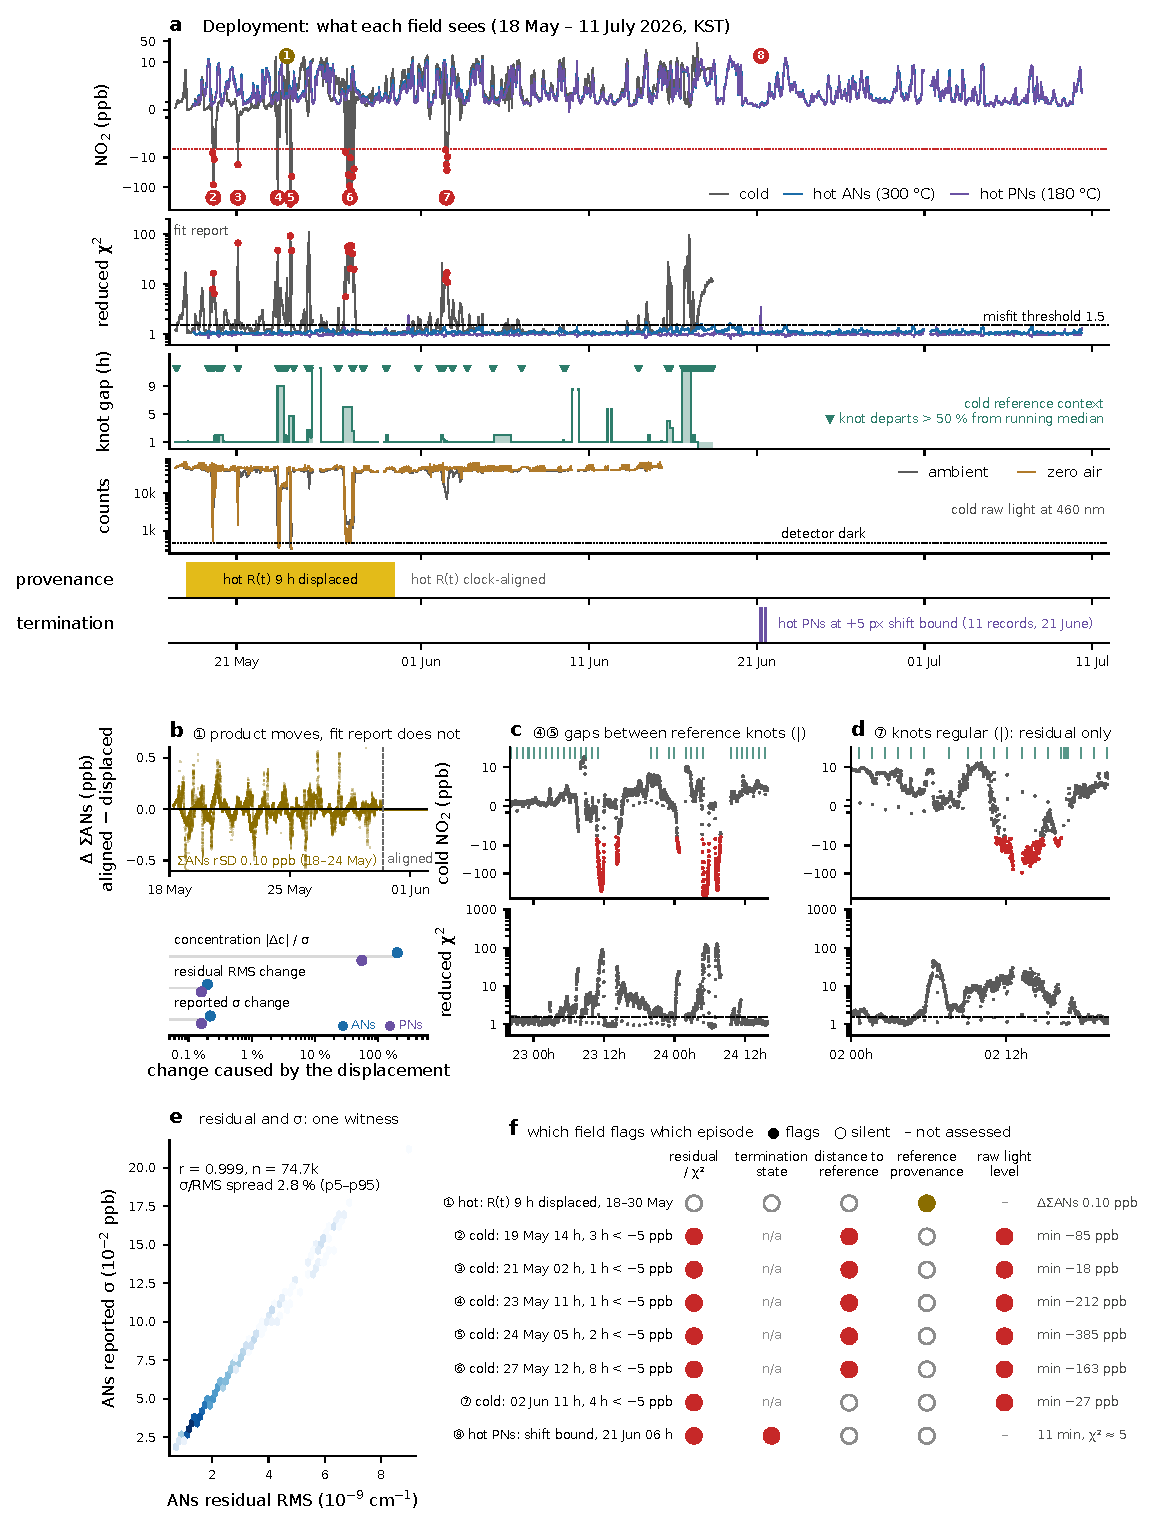
\includegraphics[width=\textwidth,height=0.62\textheight,keepaspectratio]{figures/fig06.pdf}
\caption{What each reporting field flags during the deployment (18 May -- 11 July 2026, KST).
\textbf{(a)} From top: hourly median NO$_2$ of the three configurations (symmetric-log axis; red: cold hours below
$-5$\,ppb); hourly median reduced $\chi^2$ with the misfit threshold of 1.5; for the cold channel, the interval between
the reflectivity knots that bracket each record (triangles: a knot departing by more than 50\,\% from its running
median); the raw cold-channel light at 460\,nm in ambient and zero-air spectra, with the detector dark level;
the provenance of the heated-channel reflectivity; and records that terminated at a shift bound.
Numbered badges mark the episodes of panel f. \textbf{(b)} Episode \textcircled{\scriptsize 1}: the change in $\Sigma$ANs when the heated channels are
retrieved with the clock-aligned instead of the 9\,h displaced reflectivity (points: records; line: 6\,h median;
dashed: end of the displaced span). Below, for 18--24 May, the change in concentration expressed in units of its
reported $\sigma$, against the change in residual RMS and in reported $\sigma$. \textbf{(c)} Episodes \textcircled{\scriptsize 4} and \textcircled{\scriptsize 5}: cold NO$_2$ and
reduced $\chi^2$ per record, with reflectivity knot times as ticks; the excursions fall in \fieldnum{9.0}\,h and \fieldnum{4.7}\,h gaps.
\textbf{(d)} Episode \textcircled{\scriptsize 7}: the same for 2 June, where the knots are regular and only the residual flags the records.
\textbf{(e)} Reported $\sigma$ against residual RMS for every hot ANs record. \textbf{(f)} For each episode, whether the residual
($\chi^2 > 1.5$), the termination state, the distance to the nearest reference (knot interval $>2$\,h or knot
departure $>50$\,\%), the reference provenance, or the raw light level (ambient or zero-air count below 30\,\% of its usual value) flags it;
the light level was not assessed for the heated channels (--); the cold configuration has fixed shift and squeeze, so its
termination state carries no bound information (n/a).}
\label{fig:6}
\end{figure*}
